% --------------------------------------------------------
% -*-TeX-*- -*-Soft-*- Soft Wrapping
% --------------------------------------------------------
% AMS-LaTeX Paper ****************************************
% --------------------------------------------------------
% Submitted:      Trans.Amer.Math.Soc. in February 1995
% Final Version:  July 1995
% Accepted:       June 1995
% --------------------------------------------------------
% This is a journal top-matter template file
% for use with AMS-LaTeX.
%%%%%%%%%%%%%%%%%%%%%%%%%%%%%%%%%%%%%%%%%%%%%%%%%%%%%%%%%%

\documentclass{tran-l}

%\usepackage[active]{srcltx} % SRC Specials
\usepackage{graphicx}
\usepackage{amsmath}
\usepackage{caption}
% Over-full v-boxes are due to the \v{c} in author's name
\vfuzz2pt % Don't report small over-full v-boxes

% THEOREM Environments ------------------------------------
\newtheorem{thm}{Theorem}[subsection]
\newtheorem{cor}[thm]{Corollary}
\newtheorem{lem}[thm]{Lemma}
\newtheorem{prop}[thm]{Proposition}
\theoremstyle{definition}
\newtheorem{defn}[thm]{Definition}
\theoremstyle{remark}
\newtheorem{rem}[thm]{Remark}
\numberwithin{equation}{subsection}
% MATH ----------------------------------------------------
\DeclareMathOperator{\RE}{Re}
\DeclareMathOperator{\IM}{Im}
\DeclareMathOperator{\ess}{ess}
\newcommand{\eps}{\varepsilon}
\newcommand{\To}{\longrightarrow}
\newcommand{\h}{\mathcal{H}}
\newcommand{\s}{\mathcal{S}}
\newcommand{\A}{\mathcal{A}}
\newcommand{\J}{\mathcal{J}}
\newcommand{\M}{\mathcal{M}}
\newcommand{\W}{\mathcal{W}}
\newcommand{\X}{\mathcal{X}}
\newcommand{\BOP}{\mathbf{B}}
\newcommand{\BH}{\mathbf{B}(\mathcal{H})}
\newcommand{\KH}{\mathcal{K}(\mathcal{H})}
\newcommand{\Real}{\mathbb{R}}
\newcommand{\Complex}{\mathbb{C}}
\newcommand{\Field}{\mathbb{F}}
\newcommand{\RPlus}{\Real^{+}}
\newcommand{\Polar}{\mathcal{P}_{\s}}
\newcommand{\Poly}{\mathcal{P}(E)}
\newcommand{\EssD}{\mathcal{D}}
\newcommand{\Lom}{\mathcal{L}}
\newcommand{\States}{\mathcal{T}}
\newcommand{\abs}[1]{\left\vert#1\right\vert}
\newcommand{\set}[1]{\left\{#1\right\}}
\newcommand{\seq}[1]{\left<#1\right>}
\newcommand{\norm}[1]{\left\Vert#1\right\Vert}
\newcommand{\essnorm}[1]{\norm{#1}_{\ess}}
% -----------------------------------------------------------
\begin{document}

\title[]
{Transforming risk over time and space}

\author{}

\address{}

\email{}

\thanks{}

\thanks{}

\subjclass{}

\keywords{}

\date{}

\dedicatory{}

\commby{}

% -----------------------------------------------------------


% -----------------------------------------------------------
\maketitle
% ----------------------------------------------------


\section*{Motivation}

Financial market participants are generally risk averse. Risk aversion compels them to pay higher than expected value for securities that reduce their portfolio risk. Risk sellers provide something like insurance and receive something like an insurance premium with a positive ex-ante expected value.

Much of this risk is specific and large. For example a company might wish to buy insurance against interest rate increases on a 100M floating rate loan. To find insurance the company must find a counter-parties that wishes to hedge the opposite exposure or an insurer willing to take the risk on book. The specificity of the risk can reduce the number of possible counter-parties and so increase the price.

The situation is improved if the larger security can be manufactured from smaller securities. A combination of smaller and more generic can sometimes find a larger market. Less constrained insurers will be more willing to sell insurance. More risk will be exchanged. Prices will fall.

To what extent is this decomposition of risk possible? For example: is it  possible to break up the risk of the interest rate rise next month into a series of simple bets paying \$1 or \$0 and lasting 10 seconds? Yes it is.

This note demonstrates simple procedures to transform the risk profile. Risky securities can be combined across time -- so a longer maturities can be manufactured from a series of shorter maturities; and structurally -- so the payoff profile can be twisted or flattened to any function of an unknown future price. The first section establishes these transforms, the second section gives some examples of widely traded risky securities that might be candidates. The final section gives a simulated example. 

\section*{Basic transforms}

\subsection*{The Universe}

\begin{itemize}
\item We exist at time $0$ with a price $S(0)$. Basic object is a price $S(T)$ which is a random variable that can take any value on $(0,\infty)$ at a future time $T>0$.
\item A binary option pays \$1 if $S(T)$ is above or equal to $K$ and \$0 if $S(T)$ is less than $K$. Call this $B_{K,T}(0)$.
\item A call option pays $\max(S(T)-K,0)$. Call this $C_{K,T}(0)$.
\item Binaries and calls exist and are tradable in any quantity for all $K$ and $T$.
\item Interest rate is 0. 
\end{itemize}

Under these conditions the price of a binary $B_{K,T}(0)$ is the market implied probability that the price will exceed $K$ at time $T$. A full set of binaries provides a full probability distribution of the price at any point in time.

\subsection*{Transforms}

\subsubsection*{Structural transformations with binaries:}

\textbf{Claim:} It is possible to create any payoff function $f(S(T))$ with binaries. For example we could use binaries to create a payoff $\sin(S(T)^2)$. Or whatever.

\textbf{Proof:} Consider $+B_{K_1} - B_{K_2}$. This makes a block with height 1 and width $K_2-K_1$. Now consider $\alpha B_K$; this makes a binary with height $\alpha$. We can therefore make any block of arbitrary height and width.  Such blocks are capable of constructing any function of $S(T)$ in limiting cases.

(note this we can also create a call since a call is a function of S(T))

\subsubsection*{Structural transformations with calls:}

\textbf{Claim:} It is possible to can create any payoff function $f(S(T))$ with calls.

Proof: Consider $+C_{K_1}-C_{K_2}$,  $K_2>K_1$. As $K_1 \rightarrow K_2$ the payoff is proportional to a binary. This can be scaled to a normal 0/1 binary. Binaries can make any function of $S(T)$.

\subsubsection{Temporal transformations with binaries:}

We can create a binary $B_{K,T_2}$ as a transform of claims on shorter maturity binaries:

\begin{itemize}
\item At $t=0$ buy $B_{K,T_1}$ 
\item At $t=T_1$ $S(T_1)\geq K$ buy a security that pays $B_{K,T_2} -1$ otherwise buy $B_{K,T_2}$
\end{itemize}

The total transaction has the same payoff at $T_2$ as the $B_{K,T_2}$ binary purchased at time 0.

\subsubsection*{Temporal transformations with calls:}

We can create a call $C_{K,T_2}(0)$ as a combination of shorter maturity calls $C_{K,T_1}(0)$, $C_{S(T_1),T_2}(T_1)$, and $C_{K,T_2}(T_1)$

\begin{itemize}
\item At $t=0$ buy $C_{K,T_1}(0)$
\item At $t=T_1$ if $S(T_1)\geq K$  buy $C_{S(T_1),T_2}(T_1)$ otherwise buy $C_{K,T_2}(T_1)$
\end{itemize}

The total transaction has the same payoff at $T_2$ as the $C_{K,T_2}(0)$

Structural and temporal risk transforms of this type can create any payoff function $f(S(T))$ as a combination of securities with maturities less than $T$.

\section*{Candidate risky securities}

\begin{itemize}
\item Call structures on equities/currencies/commodities/interest rates/CDS. Especially at the money options close to expiry as these generally have a higher volatility premium.
\item Swaps or forwards where the swap rate or forward price incorporates a risk preference from the buying or selling side (e.g electricity, dividend swaps, VIX futures, weather, earthquake, etc)
\item Guaranteed execution prices: Market participants will often cross the bid-offer spread to make a trade. Under normal circumstances the expected price should be the mid-point between the bid and the ask. The additional spread is paid as a type of insurance against missing an order. This risk has a call structure  and can easily be decomposed.
\end{itemize}

These can be sold on exchange or OTC and hedged with smaller and shorter dated calls or binaries. In each case it's not necessary to replicate the whole security. The risk can be held and replicated at any time and then bought back from the market before expiry/maturity.

\section*{Simulated example}

We have a one month interest rate call (called a `cap') with a strike price of 5\% and an annualised implied volatility of 2\% on a 100M notional value. The replicating portfolio is constructed as a series of calls each 10 seconds constructed as above.

The simulation creates a series of interest rates each 10 seconds for 30 days with 2\% annualised realised volatility. The histogram in figure \ref{fig:callReplicationHist} is the distribution payoffs to each of the 259,200 calls used to hedge the larger option.


 \begin{center}
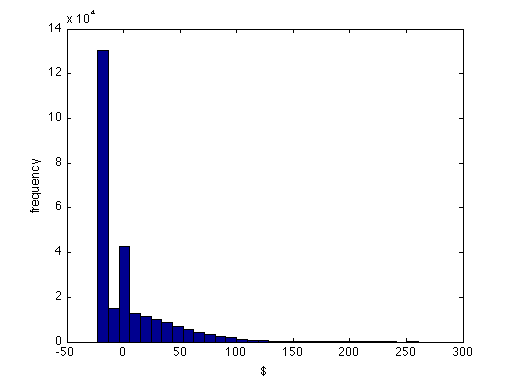
\includegraphics[width=6in]{pics/callReplicationHist}%
\captionof{figure}{Payoff distribution for 10 second calls}
\label{fig:callReplicationHist}%
\end{center}

\begin{center}
\begin{tabular}{|c|c|}
\hline
mean & 0 \\
std & \$31 \\
max &\$22 \\
min &\$-260 \\
\hline
\end{tabular}
\end{center}

The price of the 30 day option would be \$11,437. The price of the 10 second options averages \$20. The maximum loss on any trade in the simulation holding the full 100M option risk for 10 seconds is \$260.

This kind of replication process can be adjusted to cap the maximum loss from each smaller bet by also buying calls slightly above the strike. In this case the payoff distribution is capped and similar to a construction from 10 second binaries.  


\end{document}




